% !TeX program = xelatex
\documentclass{article}
\usepackage[paperwidth=155mm,paperheight=230mm,margin=18mm]{geometry}
\usepackage{fontspec,xeCJK,graphicx,xcolor,tikz}
\usepackage[absolute,overlay]{textpos}
\usepackage[unicode,pdfpagelayout=TwoPageLeft,pdftitle={阿尔刻提斯之歌 · 中英对照剧本}]{hyperref}
\setmainfont{texgyrepagella-regular.otf}[
  ItalicFont=texgyrepagella-italic.otf,
  BoldFont=texgyrepagella-bold.otf,
  BoldItalicFont=texgyrepagella-bolditalic.otf]
\IfFileExists{/usr/local/share/fonts/f/FZShuSong_Z01_Regular.ttf}{
  \setCJKmainfont{FZShuSong_Z01_Regular.ttf}[Path=/usr/local/share/fonts/f/,ItalicFont=FZKai_Z03_Regular.ttf]
  \newCJKfontfamily\kai{FZKai_Z03_Regular.ttf}[Path=/usr/local/share/fonts/f/]
  \newCJKfontfamily\hei{FZHei_B01_Regular.ttf}[Path=/usr/local/share/fonts/f/]
}{
  \setCJKmainfont{Noto Serif CJK SC}
  \newCJKfontfamily\kai{FangSong}
  \newCJKfontfamily\hei{Noto Sans CJK SC}
}
\definecolor{ink}{gray}{.12}
\definecolor{quiet}{gray}{.40}
\pagestyle{empty}
\color{ink}
\setlength{\parindent}{0pt}
\setlength{\parskip}{0pt}
\xeCJKsetup{PunctStyle=kaiming}
\textblockorigin{0mm}{0mm}
\newcommand{\ENsetup}{\normalfont\color{ink}\fontsize{11}{16.5}\selectfont\emergencystretch=1.5em}
\newcommand{\ZHsetup}{\normalfont\color{ink}\fontsize{10.5}{17}\selectfont\emergencystretch=1.5em}
\newcommand{\ENspeaker}[1]{{\fontsize{9.8}{13}\selectfont\scshape\bfseries #1}\par\vspace{3pt}}
\newcommand{\ZHspeaker}[1]{{\hei\fontsize{10.3}{13}\selectfont #1}\par\vspace{3pt}}
\newcommand{\ENstage}[1]{\par\noindent{\itshape #1}\par}
\newcommand{\Note}[2]{\par\hangindent=1.5em\hangafter=1\noindent\makebox[1.5em][l]{#1}#2\par}
\newcommand{\Block}[3]{\begin{textblock*}{119mm}(18mm,#1mm){#2 #3\par}\end{textblock*}}
\newcommand{\Heading}[3]{%
  \begin{textblock*}{119mm}(18mm,12mm)
    \color{quiet}\fontsize{7.5}{10}\selectfont
    #1\hfill #2\par\vspace{3mm}\hrule height .2pt
  \end{textblock*}
  \begin{textblock*}{119mm}(18mm,214mm)
    \color{quiet}\fontsize{7}{10}\selectfont #3\hfill\thepage
  \end{textblock*}
}
\newcommand{\Ornament}{%
  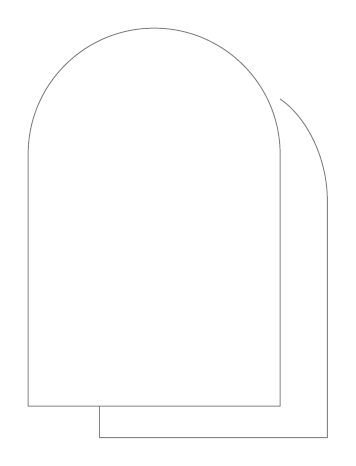
\begin{tikzpicture}[x=1mm,y=1mm,draw=ink!55,line width=.35pt]
    \draw (9,0)--(38,0)--(38,30).. controls (38,36) and (35,41)..(32,43);
    \draw (9,0)--(9,4);
    \draw (0,4)--(32,4)--(32,36) arc[start angle=0,end angle=180,radius=16]--cycle;
  \end{tikzpicture}
}

\begin{document}
\null
\begin{textblock*}{119mm}(18mm,40mm)\centering \fontsize{25}{35}\selectfont THE\\ALCESTIAD\end{textblock*}
\begin{textblock*}{119mm}(18mm,74mm)\centering\fontsize{10}{15}\selectfont THORNTON WILDER\end{textblock*}
\begin{textblock*}{119mm}(18mm,100mm)\centering\fontsize{13}{20}\selectfont FOREWORD · ACT I\par\vspace{13mm}\Ornament\end{textblock*}
\begin{textblock*}{109mm}(23mm,185mm)\centering\fontsize{10}{15}\selectfont The rear court of the palace of Admetus, King of Thessaly, many centuries before the Great Age of Greece.\end{textblock*}
\begin{textblock*}{119mm}(18mm,215mm)\centering\color{quiet}\fontsize{8}{11}\selectfont ENGLISH · CHINESE\end{textblock*}
\newpage
\null
\begin{textblock*}{119mm}(18mm,48mm)\centering \fontsize{23}{34}\selectfont 阿尔刻提斯之歌\end{textblock*}
\begin{textblock*}{119mm}(18mm,74mm)\centering\fontsize{10}{15}\selectfont 桑顿·怀尔德\end{textblock*}
\begin{textblock*}{119mm}(18mm,100mm)\centering\fontsize{13}{20}\selectfont 前言 · 第一幕节选\par\vspace{13mm}\Ornament\end{textblock*}
\begin{textblock*}{109mm}(23mm,185mm)\centering\fontsize{10}{15}\selectfont 塞萨利国王阿德墨托斯王宫的后院，\\希腊黄金时代几个世纪之前。\end{textblock*}
\begin{textblock*}{119mm}(18mm,215mm)\centering\color{quiet}\fontsize{8}{11}\selectfont 中英对照 · 节选\end{textblock*}
\newpage
\null
\Heading{THE ALCESTIAD}{FOREWORD}{Original p. ix}
% foreword-0 en
\Block{30.000}{\ENsetup}{On the last pages of Thornton Wilder's novel \textit{The Eighth Day}, my brother has one of the leading characters refute the usual image of the life experience as a river flowing onward between defined banks. Instead, the human adventure is described as a tapestry with indeterminate breadth as well as length and the individual pattern visible on both sides of the fabric. The story is outlined in colored yarn, the design perhaps wildly asymmetrical but nevertheless clear, truthful, complete. A record and a portrait.\par}
% foreword-1 en
\Block{79.514}{\ENsetup}{Thornton's tapestry was minute when at the age of seven or eight in Madison, Wisconsin, he first heard the name Alcestis while reading or being read to from Bulfinch's \textit{The Age of Fable}. The story of the daughter of King Pelias, princess of princesses in the myth and the song of pre-Christian Greece, captured his imagination—and his heart. The thread of her white yarn was knotted into his bit of fabric and she became a benign insistence in his inner consciousness, that hidden storehouse which is an author's source and springboard. She was the haunting shadow of a play that would take years to write.\par}
\newpage
\null
\Heading{阿尔刻提斯之歌}{前言}{原书 1–2}
% foreword-0 zh
\Block{30.000}{\ZHsetup}{人们总是将生命看作一条沿着既定路线奔流的河，而在桑顿·怀尔德的小说《第八日》的最后几页，我哥哥让其中一位主角反驳了这种看法。相较之下，一个人的人生经历就像一张织毯，它的长和宽都不确定，两面的纹路也不尽相同。彩色的纱线勾勒出故事的轮廓，设计上也许极不对称，却清晰、真实而完整。是记录，也是肖像。\par }
% foreword-1 zh
\Block{79.514}{\ZHsetup}{桑顿的命运织毯起初还很小，七八岁时他生活在威斯康星州的麦迪逊市，在阅读布尔凡奇的《寓言时代》时第一次听到了阿尔刻提斯这个名字。在前基督教时期的希腊神话和歌谣中，国王佩利阿斯的女儿是公主中的公主。她的故事占据了他的想象，也俘获了他的心灵。她的白色纱线嵌进了他的命运织物中，阿尔刻提斯成为他潜意识中一份温柔的坚持，一个有待发掘的灵感素材。她是一个戏剧雏形，直到多年后才得以创作出来。\par }
\newpage
\null
\Heading{THE ALCESTIAD}{FOREWORD}{Original pp. ix–x}
% foreword-2 en
\Block{30.000}{\ENsetup}{The knot in Alcestis's thread was tied when the Wilder family moved to Berkeley, California, where the magnificent Greek Theater built into the hillside of a eucalyptus grove was a new and lively part of the life of the university and the town. Several times a year the Classics Department mounted productions of plays by Sophocles, Aeschylus, and Euripides. Our mother joined the volunteer workers in the costume shop and stenciled furlongs of borders in the Greek key or laurel leaf patterns on gorgeously colored togas. She made a little blue one with shells around the hem for Thornton—and a green one for brother Amos—and sent them off to apply for roles as members of the Athenean mob. Thus Thornton discovered ``total'' theater and the Golden Age of Antiquity. His experience until then had been a performance of \textit{As You Like It} seen from the top gallery of a Milwaukee theater.\par}
% foreword-3 en
\Block{108.498}{\ENsetup}{By now Thornton was ten; black-haired, blue-eyed, acquisitive and radiant. Even before this he had claimed his share of a writer's allotment of the twenty-six letters of the alphabet and had begun to tame them into a vocabulary that would allow him—in good time—to speak in his own way. He went to bed early and got up early to write, and the full range of his enlarging vocabulary was turned to inventing dialogue. He draped us and the neighbors' children in yards of begged or borrowed cheesecloth and coaxed us into declaiming his grandiloquent speeches.\par}
% foreword-4 en
\Block{163.783}{\ENsetup}{Four years later he was a boarding pupil in the China Inland Mission School in Chefoo. Studies in the classics began early in a British school preparing its pupils for the Oxford-Cambridge Examinations.\par}
\newpage
\null
\Heading{阿尔刻提斯之歌}{前言}{原书 2–3}
% foreword-2 zh
\Block{30.000}{\ZHsetup}{当怀尔德一家搬到加利福尼亚州伯克利时，阿尔刻提斯之线打了个结。桉树林山坡上建有一座宏伟的希腊剧院，是学校和小镇生活中生机勃勃的一部分。古典学系每年都会制作几部索福克勒斯、埃斯库罗斯和欧里庇得斯的戏剧作品。我们的母亲参与了服装组的志愿工作，用模板印出希腊钥匙的形状，或是在漂亮的长袍上印上月桂树叶的图案。她给桑顿做了一件有贝壳镶边的蓝色小袍子——给哥哥阿莫斯做了一件绿色的——然后让他们去扮演雅典民众。桑顿就这样了解到了“整个”剧场和古希腊的黄金时代，在这之前，他的全部剧场经验不过是坐在密尔沃基剧院的后排看了一场《皆大欢喜》。\par }
% foreword-3 zh
\Block{108.498}{\ZHsetup}{桑顿十岁了，黑头发，蓝眼睛，充满好奇心，精力旺盛。早在十岁之前他就掌握了作家们的工具，驯服了二十六个字母为自己服务，将它们组成词汇，在适当的时候用来表达自己。他早睡早起写作，随着词汇量的增长，他开始创造对话。他给我们和邻居的孩子披上借来的纱，哄着我们一起朗诵他的豪言壮语。\par }
% foreword-4 zh
\Block{163.783}{\ZHsetup}{四年之后，他成为中国烟台一所教会学校的寄宿生。在一所英国人开办的专为牛津、剑桥入学考试做准备的学校里，他开始了对古典文学的学习。\par }
\newpage
\null
\Heading{THE ALCESTIAD}{FOREWORD}{Original pp. x–xi}
% foreword-5 en
\Block{30.000}{\ENsetup}{The first half of his undergraduate years was spent at Oberlin College in Ohio, where he became a privileged student and friend of a great teacher who was also a distinguished classicist—Professor Charles H. A. Wager. Alcestis's thread wove a visibly increasing pattern during these years and later, following his graduation from Yale in 1920, when he spent eight months at the American Academy for Classical Studies in Rome. Not qualified as a Graduate Fellow, he nevertheless audited lectures, went on digs with the archaeologists and pored over fragile papyri. In the museums and art galleries of Italy he caught Alcestis's shadow.\par}
% foreword-6 en
\Block{90.084}{\ENsetup}{In the decades of the twenties and the thirties the tapestry grew in size and density. The design was of teaching—first French at The Lawrenceville School and then comparative literature, including the Greek dramatists, at the University of Chicago—and lecture tours and script-writing in Hollywood. He published two volumes of short plays and four novels. One, \textit{The Bridge of San Luis Rey}, brought him the first of three Pulitzer Prizes and, at the age of thirty, world-wide fame weighted with a cumbersome bag of perquisites: honors, privileges, dazzling opportunities balanced by loss of privacy and hazards to body, mind, and spirit.\par}
% foreword-7 en
\Block{151.184}{\ENsetup}{During these years the first of Thornton's long plays, \textit{Our Town}, was produced to immediate success, and the second, \textit{The Merchant of Yonkers}, to failure. André Obey's play, \textit{Lucrèce}, which Katharine Cornell had commissioned my brother to translate for her, opened and closed while Ibsen's \textit{A Doll's House}, adapted by him for Ruth Gordon, was a conspicuous success.\par}
\newpage
\null
\Heading{阿尔刻提斯之歌}{前言}{原书 3–4}
% foreword-5 zh
\Block{30.000}{\ZHsetup}{他大学时代的前两年是在俄亥俄州的欧伯林学院度过的。在那里他成了查尔斯·H. A. 瓦格教授的得意门生和朋友，而瓦格教授本身也是一名出色的古典文学家。1920 年从耶鲁大学毕业后，他在美国设立于罗马的古典学研究院待了八个月，阿尔刻提斯之线在这些年里有了更清晰的纹路。尽管不是一名研究员，他还是会去听讲座，和考古学家们一起去挖掘现场，仔细研读莎草纸上的文字。在意大利的博物馆和美术馆里，他捕捉到了阿尔刻提斯的影子。\par }
% foreword-6 zh
\Block{90.084}{\ZHsetup}{在二十世纪二三十年代里，这张命运织毯延展得更大，也变得更加密实。他开始从事教学工作——先是在劳伦斯维尔学校教授法语，然后在芝加哥大学教授比较文学，其中也会讲到古希腊的剧作家们——还有巡回演讲以及在好莱坞进行电影剧本创作。他出版了两部短剧集和四部小说，其中一部《圣路易斯雷大桥》为他赢得了普利策奖，在三十岁的这一年使他名扬四海。随之而来的是各种特权、荣誉和令人眼花缭乱的机遇，同时他也失去了很多隐私，身体、思想和精神都受到了危害。\par }
% foreword-7 zh
\Block{151.184}{\ZHsetup}{这几年里，桑顿的第一部长剧《我们的小镇》在制作演出后便取得了成功。第二部剧《扬克斯商人》则以失败告终。安德烈·奥比的剧作《卢克丽丝》由凯瑟琳·康奈尔委托给我哥哥翻译，这部剧开演后又停演。与此同时，他帮鲁斯·戈登改编的易卜生的《玩偶之家》则取得了巨大的成功。\par }
\newpage
\null
\Heading{THE ALCESTIAD}{FOREWORD}{Original pp. xi–xii}
% foreword-8 en
\Block{30.000}{\ENsetup}{In the summer of 1939 Thornton returned home wonderfully free at last of all outside commitments, with his head full of plans for his own work. He had the beginnings of two projects, both plays. One did not have a name yet. The other was \textit{The Alcestiad}. September came and Hitler's armies flooded Holland and Belgium. Thornton had no choice; \textit{The Alcestiad} was not a play for a war-torn world. The untitled project which became \textit{The Skin of Our Teeth} was.\par}
% foreword-9 en
\Block{73.676}{\ENsetup}{Soon after Pearl Harbor Thornton was commissioned a captain in the Air Force. By strange coincidence his final leave before going overseas came at the time of the previews and opening of \textit{The Skin of Our Teeth} in New York. The morning that Mother and I said goodbye to him he patted his bulging duffle bag. ``I have the manuscript of \textit{The Alcestiad} in my kit. I've been thinking how I could make it into a good one-act. It's very possible by using just the big second act scene. I'd like to leave a finished piece of work . . . might come in handy, Mother. It's a toss-up if \textit{The Skin of Our Teeth} will catch on. . . .''\par}
% foreword-10 en
\Block{128.950}{\ENsetup}{Two years later, while he was waiting in a camp near Boston to be separated from the Air Force (a lieutenant colonel now), his papers were lost. The commanding officer of the post offered a three-day pass. Thornton went straight from the Back Bay station to the Boston Public Library on Copley Square, where he drowned himself once more in the Golden Age of Greece. A few days later he was for the first time in more than three years seated at his own desk in Hamden, Connecticut.\par}
\newpage
\null
\Heading{阿尔刻提斯之歌}{前言}{原书 4–5}
% foreword-8 zh
\Block{30.000}{\ZHsetup}{1939 年夏天，桑顿终于完成了所有的邀约工作，带着完全自由的状态和满腹个人创作计划回到家中。他已经写了两部作品的开头，两部都是戏剧。一部还没有命名，另一部就是《阿尔刻提斯之歌》。九月到了，希特勒的军队横扫了荷兰和比利时，桑顿别无选择。《阿尔刻提斯之歌》并不适合一个战乱的世界。此时尚未被命名的《九死一生》才更合适。\par }
% foreword-9 zh
\Block{73.676}{\ZHsetup}{珍珠港事件后，桑顿被任命为空军上尉。很巧的是，他出国服役前的最后一天，正是《九死一生》在纽约首演的日子。我和母亲同他告别的那个早上，他拍了拍自己鼓鼓的行囊说道：“我打包了《阿尔刻提斯之歌》的手稿在里面。我一直在琢磨把它写成一个不错的独幕剧，很可能只需要第二幕的那一大场戏。我想留下一部完成的作品……说不定能派上用场，妈妈。《九死一生》能不能成功也说不定呢……”\par }
% foreword-10 zh
\Block{128.950}{\ZHsetup}{两年后，他弄丢了自己的手稿。彼时他已经是一位空军中校，正在波士顿附近的军营里等待着退伍。指挥官批准他离开三天，桑顿从后湾车站直奔科普利广场的波士顿图书馆，再次沉浸到了古希腊的黄金时代之中。几天后，他终于在三年后又一次坐在了康涅狄格汉姆登自己的书桌前。\par }
\newpage
\null
\Heading{THE ALCESTIAD}{FOREWORD}{Original pp. xii–xiii}
% foreword-11 en
\Block{30.000}{\ENsetup}{A single sheet of paper from that time is before me now. Printed on one side in big block letters is:\par}
% foreword-12 en
\Block{44.708}{\ENsetup}{\centering 
THE ALCESTIAD\par
A PLAY OF QUESTIONS\par}
% foreword-13 en
\Block{59.012}{\ENsetup}{On the reverse in his small careful penmanship is:\par}
% foreword-14 en
\Block{67.913}{\ENsetup}{\leftskip=4mm\rightskip=3mm 
(Sketches up to and including the Tiresias scene of Act One had been made before the War and lost)\par
Draft One of the first act, May and July 1945\par
Draft Two, begun July 8, 1945\par
This Draft Three begun (after completion of Act II and half of Act III) on Dec\par}
% foreword-15 en
\Block{105.728}{\ENsetup}{The unfinished date would be 1945.\par}
% foreword-16 en
\Block{114.188}{\ENsetup}{The loss of the manuscript meant more to my brother than these few notes convey; his eagerness to get back to his peacetime profession fired his enthusiasm and carried him along for the seven months of work recorded here. But, like millions of other soldiers, he had returned home not only a disoriented and exhausted man but a changed one. He was not able easily to recapture his prewar vision of Alcestis and he did not have the reserve of physical and nervous energy to sustain the excitement and tension to finish his work. He found he was beginning to destroy rather than build. Fortunately he recognized this and put the manuscript away again before doing it injury.\par}
\newpage
\null
\Heading{阿尔刻提斯之歌}{前言}{原书 5–6}
% foreword-11 zh
\Block{30.000}{\ZHsetup}{此刻我面前正放着那时他留下的一张纸，一面用大写字母打印着：\par }
% foreword-12 zh
\Block{44.708}{\ZHsetup}{\centering\kai 《阿尔刻提斯之歌》\par 一出充满问题的戏剧\par }
% foreword-13 zh
\Block{59.012}{\ZHsetup}{反面是他写的一些小字：\par }
% foreword-14 zh
\Block{67.913}{\ZHsetup}{\leftskip=4mm\rightskip=3mm\kai {\kai （第一幕戏的草稿，包括有忒瑞西阿斯的场景，都在战争前完成，已经遗失）}\par 第一幕初稿，1945 年 5 月和 7 月\par 第二稿，1945 年 7 月 8 日开始创作\par 第三稿，12 月开始{\kai （在第二幕与第三幕的一半完成后）}\par }
% foreword-15 zh
\Block{105.728}{\ZHsetup}{没写上的日期应该是 1945 年。\par }
% foreword-16 zh
\Block{114.188}{\ZHsetup}{遗失手稿给哥哥带来的影响远不是这几行笔记可以传达的。他急切地想要回到和平时期的状态中，这激发了他的热情，让他如记录中所写的样子，连续创作了七个月的时间。然而，就如同其他上百万的士兵们一样，他回到家时不只是迷茫与疲惫，整个人也完全改变了。他不再能够以战争之前那样的视角来看待阿尔刻提斯了，他的体力和精力也不足以支撑自己保持一个亢奋的状态来完成工作。他发现自己所做的更多是破坏而不是创造。好在他意识到了这一点，在造成破坏前就停止了自己的工作。\par }
\newpage
\null
\Heading{THE ALCESTIAD}{FOREWORD}{Original p. xiii}
% foreword-17 en
\Block{30.000}{\ENsetup}{Ancient literature is replete with warriors and battlefields, tyrants and heroes. My brother's thoughts were still lively with his own recent experiences of Hitler's and Mussolini's wars: one year spent on the North African coast among the ruins and ghosts of Hellenic and Roman conquest; another year in southern Italy, likewise haunted by dramatic legend, with Caesar's image triumphant. Thornton suddenly saw his next work plain. And so it happened that the novel, \textit{The Ides of March}, was written and published in 1948. It opened the way for his return to civilian life, to teaching and lecturing again, to the theater and to Alcestis.\par}
% foreword-18 en
\Block{90.084}{\ENsetup}{Thornton was only one of many authors after Euripides to be inspired to retell in his own way the Alcestis fable. Among others Christoph Martin Wieland in Germany in 1773 wrote a libretto for an operetta on the subject. In the next century the poets Richard von Hofmannstahl in Austria and Robert Browning in England used the myth. T. S. Eliot borrowed from it for an aspect of his successful play, \textit{The Cocktail Party}. And no wonder, for the theme of conjugal love and the willingness of a wife to die for her husband is an appealing and thought-provoking challenge to any author anxious to explore and praise the capabilities of humankind.\par}
\newpage
\null
\Heading{阿尔刻提斯之歌}{前言}{原书 6–7}
% foreword-17 zh
\Block{30.000}{\ZHsetup}{古代文学故事里满是战场和战士，暴君和英雄。哥哥的思绪还围绕着他自己在希特勒和墨索里尼带来的战争中的经历：他在北非待了一年，就在那些希腊与罗马帝国留下的废墟与阴影里；又在意大利南部待了一年，那里同样充满戏剧性的传说，例如恺撒的胜利。桑顿突然有了新作品的灵感，他的小说《三月十五》在 1948 年出版。这部小说开启了他回归文明世界的道路，他又开始教书，演讲，上剧场，重新思考阿尔刻提斯的故事。\par }
% foreword-18 zh
\Block{90.084}{\ZHsetup}{在欧里庇得斯之后，有许多作家想要以自己的方式改编阿尔刻提斯的故事。1773 年，克里斯托夫·马丁·维兰德以此为题创作了一部歌剧剧本。在十九世纪，奥地利诗人胡戈·冯·霍夫曼斯塔尔和英国作家罗伯特·勃朗宁也都选取过这个题材。T. S. 艾略特在他成功的剧作《鸡尾酒会》中也有所借用。也难怪，这个故事的主旨是夫妻之间的爱，以及妻子愿意为了丈夫而死。这对任何想要发掘和赞美人类能动性的作者来说，都是充满吸引力且发人深省的挑战。\par }
\newpage
\null
\Heading{THE ALCESTIAD}{FOREWORD}{Original pp. xiii–xiv}
% foreword-19 en
\Block{30.000}{\ENsetup}{After the success at the 1954 Edinburgh Festival of \textit{The Matchmaker}—that happy invention which started its career as the New York failure \textit{The Merchant of Yonkers} and went on to become the basis of the musical comedy hit, \textit{Hello, Dolly!}—the producers commissioned from my brother a new play for the next season. This gave him the impetus needed to finish \textit{The Alcestiad}. He went into hiding at Aix-en-Provence for a long working period. At Christmas he joined a group of friends and me at Villars, Switzerland, for two weeks. During that time I typed from the manuscript the first two acts of the new text. He submitted them at once to the Festival Committee. They and Tyrone Guthrie accepted the play for their 1955 program. Before leaving Aix in the spring he sent in Act Three.\par}
% foreword-20 en
\Block{101.701}{\ENsetup}{A performance of the Classic Attic theater consisted of a trilogy of more or less connected tragedies usually followed by a Satyr play—a humorous or biting comment using characters and situations from the preceding dramas. Euripides, the youngest of the three major rival playwrights, sometimes broke with tradition by writing a single play that could stand alone or be grouped with others to complete the three-part pattern. His \textit{Alcestis} is one of these. In fact, because of its ``happy ending,'' with the heroine brought back from the underworld by Hercules, \textit{Alcestis} was even used occasionally as a Satyr play.\par}
% foreword-21 en
\Block{157.002}{\ENsetup}{My brother's first idea for his version of the story was to commission a new translation of Euripides's text for a middle act and write a first and third to frame it. Soon he discarded the plan as not practical for his purposes.\par}
\newpage
\null
\Heading{阿尔刻提斯之歌}{前言}{原书 7–9}
% foreword-19 zh
\Block{30.000}{\ZHsetup}{1954 年，《媒人》在爱丁堡艺术节上演并获得成功——这部有趣的作品由纽约的失败之作《扬克斯商人》而来，后来发展成为大热的音乐剧《你好，多莉！》——制作人委托我哥哥为下一季创作新作品，这给了他完成《阿尔刻提斯之歌》的动力。他在普罗旺斯的艾克斯闭关创作了很长一段时间。圣诞节时，他聚集了包括我在内的一帮朋友，一起在瑞士的维拉斯待了两周。在此期间，我依据他的手稿打出了新文本的前两幕，他立刻提交给了艺术节组委会。泰隆·格思里接受这出戏参与到 1955 年的节日中，春天离开艾克斯之前，他提交了第三幕。\par }
% foreword-20 zh
\Block{101.701}{\ZHsetup}{古希腊剧场的演出由内容相关联的悲剧三部曲组成，通常还有一出羊人剧\textsuperscript{1}——用前面剧中的人物和情节进行或幽默或尖锐的注解。欧里庇得斯是三大对手剧作家中最年轻的一位，他有时会打破传统，写一部可以独立上演的剧本，或者该剧可以与其他剧目组合成为三部曲。他的《阿尔刻提斯》就是这个类型的剧目之一。事实上，由于它的“大团圆结局”——女主角被赫拉克勒斯从冥界带回人间，《阿尔刻提斯》偶尔甚至会被用作羊人剧演出。\par }
% foreword-21 zh
\Block{157.002}{\ZHsetup}{我哥哥对于他这版改编的第一个想法，是将欧里庇得斯的文本进行全新翻译作为中间一幕，然后创作第一幕和第三幕把第二幕框起来。很快他就放弃了这个计划，因为这不符合他的目的。\par }
\begin{textblock*}{119mm}(18mm,193.967mm)\color{ink}\rule{30mm}{.25pt}\end{textblock*}
\begin{textblock*}{119mm}(18mm,197.967mm)\normalfont\color{ink}\fontsize{7.5}{11}\selectfont \Note{1}{羊人剧，是一种轻松的笑剧，不是喜剧。一般在三部悲剧上演后进行演出， 作为一种调剂。——译者注}\end{textblock*}
\newpage
\null
\Heading{THE ALCESTIAD}{FOREWORD}{Original pp. xiv–xv}
% foreword-22 en
\Block{30.000}{\ENsetup}{In the Greek telling of the legend and Bulfinch's account centuries later, King Admetus knows that he can be saved from death if another will die for him. He goes begging the favor among his servants, former military colleagues, and friends to no avail. Next, he beseeches his parents relentlessly, pointing out that since they have so few years of living left, it is a little thing to ask. But neither the old father nor the old mother is willing to give up a breath for the son. The King does not request this sacrifice of his Queen; when Alcestis offers her life with all her love his protests seem mild and unworthy.\par}
% foreword-23 en
\Block{85.301}{\ENsetup}{Thornton, by having Admetus unaware that he can be saved by another's death, gains a very dramatic and human emotional peak in act two, and deepens the characterizations and relationship of husband and wife, enriching the bare outlines of the legend for our twentieth century understanding. Concerning his version my brother has said:\textsuperscript{2}\par}
% foreword-24 en
\Block{117.398}{\ENsetup}{\leftskip=4mm\rightskip=3mm 
On one level my play recounts the life of a woman—of many women—from bewildered bride to sorely tested wife to overburdened old age. On another level it is a wildly romantic story of gods and men, of death and hell, of resurrection of great loves and great trials, of usurpation and revenge. On another level, however, it is a comedy . . . about the extreme difficulty of any dialogue between heaven and earth, about the misunderstandings that result from the incommensurability of things human and divine.\par}
\begin{textblock*}{119mm}(18mm,189.932mm)\color{ink}\rule{30mm}{.25pt}\end{textblock*}
\begin{textblock*}{119mm}(18mm,193.932mm)\normalfont\color{ink}\fontsize{7.5}{11}\selectfont \Note{2}{Quoted by Paul M. Cubeta in \textit{Modern Drama for Analysis} (New York: Holt, Rinehart \& Winston, Inc., 1955), pp. 595–596.}\end{textblock*}
\newpage
\null
\Heading{阿尔刻提斯之歌}{前言}{原书 9–10}
% foreword-22 zh
\Block{30.000}{\ZHsetup}{在希腊人讲述的传说和几个世纪后布尔凡奇的记录中，阿德墨托斯国王知道，如果有人愿意为他而死，他就可以活下去。他向他的仆人、昔日的军中同僚和朋友们求救，但无济于事。而后，他不遗余力地恳求他的父母，指出既然他们的寿命所剩无几，请求他们代死只是小事一桩。但无论是老父亲还是老母亲，都不愿意为儿子放弃生命。国王没有请求他的王后做出这个牺牲，当阿尔刻提斯带着爱献出她的生命时，他的抗议显得不温不火，毫无意义。\par }
% foreword-23 zh
\Block{85.301}{\ZHsetup}{桑顿让阿德墨托斯不曾得知自己可以通过他人的死亡得到拯救，在第二幕造就了一个戏剧性和情感的高潮，并深化了人物形象和夫妻关系，为这个传说原本简单的故事线赋予了来自二十世纪的丰富解读。关于他的这个版本，哥哥说过：\par }
% foreword-24 zh
\Block{117.398}{\ZHsetup}{\leftskip=4mm\rightskip=3mm\kai 从某个层面上来说，我的剧本描述了一个女人——许多女人——从一个犹疑的新娘成长为经受着苦考验的妻子，最后成为不堪重负的老人。在另一个层面上，它是一个关于神和人，关于死亡和冥界，关于伟大的爱和伟大的试炼后的复活，关于篡夺和复仇的疯狂而浪漫的故事。在又一个层面上，它是一部喜剧……关于天界和人间沟通上的极端困难，关于人类和神明的不可比性所造成的误解。\textsuperscript{2}\par }
\begin{textblock*}{119mm}(18mm,190.214mm)\color{ink}\rule{30mm}{.25pt}\end{textblock*}
\begin{textblock*}{119mm}(18mm,194.214mm)\normalfont\color{ink}\fontsize{7.5}{11}\selectfont \Note{2}{引自保罗·M. 库贝塔的《现代戏剧分析》{\kai （纽约：霍尔特，莱因哈特和温斯顿公司， 1955）}，第 595—596 页。}\end{textblock*}
\newpage
\null
\Heading{THE ALCESTIAD}{FOREWORD}{Original pp. xv–xvi}
% foreword-25 en
\Block{30.000}{\ENsetup}{Of Thornton's other works, his third novel, \textit{The Woman of Andros}, published in 1930, comes closest in setting, feeling, and ideas to \textit{The Alcestiad}. Laid on a small Grecian island when Alcestis was already a legend, it is a nostalgic, quiet yet passionate prose-poem, a bridge with one end mired in the mud of the cruel pagan world, the other straining toward a slowly rising dawn of release. The heroine, Chrysis, is beautiful, intelligent, and has some education, but her profession as a \textit{heitara} makes her an outcast. Nevertheless, she is spiritual sister to the Queen Alcestis.\par}
% foreword-26 en
\Block{84.304}{\ENsetup}{In both these female characters Thornton pays his \textit{hommage} to all women, giving them the burden of carrying his message. Chrysis in her living and her dying praises all life—``the bright and the dark''—and teaches others to do likewise. She is unknowingly a prophet, pointing ahead to a higher hope for humanity.\par}
% foreword-27 en
\Block{116.428}{\ENsetup}{Alcestis, of course, had been entrusted with messages and heaped with laurel wreaths long before Thornton heard her name. In his play, brought back from hell to live again in the Golden Light of Apollo, she is not permitted a human end. The God steals her from Death and insists upon her perpetual life. He steals her from Admetus, thus denying her—and the king—a stela at his side in the royal tomb. Apollo leads her to His Evergreen Grove where she still wanders, a symbol, a myth, a truth for us all: one who escaped from darkness to be herself a light on the horizon comprehensible to the spirit of Christian humanism.\par}
\newpage
\null
\Heading{阿尔刻提斯之歌}{前言}{原书 10–11}
% foreword-25 zh
\Block{30.000}{\ZHsetup}{在桑顿的其他作品中，1930 年出版的第三部小说《安德罗斯的女人》在设定、情感和思想上与《阿尔刻提斯之歌》最为接近。故事发生在希腊的一个小岛上，彼时阿尔刻提斯已经成为传说。这部作品是一首怀旧的、宁静却也充满激情的散文诗，它像一座桥，一端陷在残酷的异教世界的泥沼中，另一端延伸向正缓缓到来的解放的黎明。女主角克里西丝漂亮、聪明，受过一定的教育，但因为自己交际花的身份被边缘化。然而，她是阿尔刻提斯女王精神上的姐妹。\par }
% foreword-26 zh
\Block{84.304}{\ZHsetup}{通过这两个女性角色，桑顿向所有女性表达了敬意，也让角色承担起传递自己主旨的重任。克里西丝在她的生和死中都赞颂了全部生命——“光明抑或黑暗”——并教导其他人也要这样做。她在不自知的情形下成了一位先知，为人类指明了更高的希望所在。\par }
% foreword-27 zh
\Block{116.428}{\ZHsetup}{当然，阿尔刻提斯这个名字，早在桑顿听说她之前，就已经承载了许多意义，被月桂花环围绕。在他的剧中，阿尔刻提斯从冥界被带回，重新生活在阿波罗的光芒之中，她的结局也与人类不同。神把她从死神那里偷了回来，坚持要她永远活着。阿波罗将她从阿德墨托斯身边偷走，也夺去了她——以及国王为她在皇家陵墓中立碑的机会。阿波罗把她带到自己的长青林中，她仍在那里徘徊，成为一个象征，一个神话，一个讲给我们所有人的真理：在基督教人文主义精神看来，一个逃离了黑暗的人，她自己就是地平线上的一束光。\par }
\newpage
\null
\Heading{THE ALCESTIAD}{FOREWORD}{Original p. xvi}
% foreword-28 en
\Block{30.000}{\ENsetup}{A play written in the form of ancient Greek drama should logically be performed in the traditional classic manner, in a setting of marble columns under a sun-lighted blue sky. Thornton wrote his \textit{Alcestiad} so that it could be accommodated to the conventional theater of the proscenium arch. At Edinburgh it was presented under still other circumstances, in the vast barn of a building known as The Church of Scotland Assembly Hall, box-shaped with rows and rows of uncomfortable seats facing three directions—a perfect setting for stormy sessions of factions warring over church politics and church dogma.\par}
% foreword-29 en
\Block{85.301}{\ENsetup}{In this uncongenial place the simple storytelling script of \textit{The Alcestiad} had to be blown up to near-pageantry proportions. There were not the words to cover the added action and the crowd scenes that filled the stage and trailed down the aisles under Tyrone Guthrie's exciting but overdramatic direction. Good or bad the play was nearly lost.\par}
% foreword-30 en
\Block{117.426}{\ENsetup}{Even the title was changed to \textit{A Life in the Sun}, which the management thought would have ``more box-office appeal.'' Thornton refers to this in a letter from Scotland to our brother Amos in Cambridge, Massachusetts:\par}
% foreword-31 en
\Block{142.734}{\ENsetup}{\leftskip=4mm\rightskip=3mm 
That's \textit{The Alcestiad}, but the entrepreneurs hate that for a title. . . . \textit{A Life in the Sun} is a pretty cheery title for a play fraught with dire events, but it says that Alcestis's life is rooted in Apollo and there's a deal about his being the Sun, so there you are. . . .\par}
\newpage
\null
\Heading{阿尔刻提斯之歌}{前言}{原书 11–12}
% foreword-28 zh
\Block{30.000}{\ZHsetup}{一部以古希腊戏剧形式写下的戏剧，理论上应该以传统的古典形式在一个大理石建造的露天剧场中演出。桑顿创作这版《阿尔刻提斯之歌》，也是为了它能够适应传统的镜框式舞台。在爱丁堡，这出戏的演出环境有所不同，是在一个叫作苏格兰教会大会堂的巨大谷仓里进行表演的。剧院呈箱形，一排排并不舒适的座位构成了一个三面舞台——若是要为教会政治和教会条例而在会议上互相争斗，这倒是个完美的环境。\par }
% foreword-29 zh
\Block{85.301}{\ZHsetup}{在这个不大合拍的演出环境中，《阿尔刻提斯之歌》这个简单的故事不得不被放大到一个夸张的比例。泰隆·格思里导演的处理激动人心却过度戏剧化了，他增加了舞台行动，用群戏场面填满舞台和过道。且不说是好是坏，这出戏的本质完全丧失了。\par }
% foreword-30 zh
\Block{117.426}{\ZHsetup}{甚至连剧名都改成了《阳光下的一生》，委员会认为这个名字“更具票房吸引力”。桑顿从苏格兰给身在麻省剑桥的哥哥阿莫斯写的信中提到了这一点：\par }
% foreword-31 zh
\Block{142.734}{\ZHsetup}{\leftskip=4mm\rightskip=3mm\kai 这就是《阿尔刻提斯之歌》，但老板们不想用这个名字。对于一出充满了可怖情节的戏来说，《阳光下的一生》这个名字过于轻松愉快了，但他们说阿尔刻提斯的生命源于阿波罗，而阿波罗就是太阳，所以就有了这个名字……\par }
\newpage
\null
\Heading{THE ALCESTIAD}{FOREWORD}{Original pp. xvi–xvii}
% foreword-32 en
\Block{30.000}{\ENsetup}{There were compensations for Thornton. He was not one to despair, nor even fret long. Guthrie's extraordinary talents lighted up some passages, the rare Irene Worth headed a strong cast, and most of the public seated in those uncomfortable rows were gratifyingly responsive and definite in their approval, although the critics, as they do more often than not, veered from appreciative interest and understanding to omniscient disdain.\par}
% foreword-33 en
\Block{72.686}{\ENsetup}{Most important of all, the author saw his work as a living whole in three-dimensional form. He learned what he had or had not accomplished to his own satisfaction. He also received balm for having felt betrayed by The Church of Scotland Assembly Hall when Tyrone Guthrie very magnanimously confided to him, ``I did not serve your play well.''\par}
% foreword-34 en
\Block{110.590}{\ENsetup}{There was much interest among theatrical producers in this country and elsewhere in obtaining the rights for a New York production. My brother had his own ideas as to what changes he wished to make in the text. He talked with a number of directors and listened to their suggestions. He began working on revisions. This always was difficult for him; he was at his best living in the present and looking into the future. Too many people were giving him advice, crowding him. ``I need a longer perspective,'' he told them. He withdrew the script from circulation, refusing acting rights to those who were willing to try it out as it stood.\par}
\newpage
\null
\Heading{阿尔刻提斯之歌}{前言}{原书 12–13}
% foreword-32 zh
\Block{30.000}{\ZHsetup}{桑顿还是得到了一些补偿。他不是一个会绝望的人，甚至也不会焦虑太久。格思里的才华创造了一些精彩段落，以艾琳·沃思为首的是一个强大的演员阵容。尽管批评家们还是老样子，先是充满兴趣与理解，随即便是因全知而不屑。而大部分的观众尽管坐在很不舒服的位置上，但都给出了积极的反响和明确的肯定。\par }
% foreword-33 zh
\Block{72.686}{\ZHsetup}{最重要的是，作者看到自己的作品立体而生动地呈现了出来，他知道自己做到了哪些，又有哪些不足。当泰隆·格思里非常有雅量地向他吐露“我没有把你的戏演好”时，桑顿也得到了安慰，他觉得是被苏格兰教会大会堂这个场地给坑了。\par }
% foreword-34 zh
\Block{110.590}{\ZHsetup}{国内外有许多戏剧制作人对这部作品感兴趣，想获得授权在纽约制作。哥哥对于他想要在文本上进行的调整也有自己的想法。他与一些导演进行了交流，听取了各种建议，开始着手修改。这对他来说一直不是件容易的事，他擅长的是活在当下，着眼于未来。有太多人围着他给他建议，于是他告诉他们：“我需要更长远的考量。”他收回了剧本，拒绝了那些想要基于此版本制作的请求。\par }
\newpage
\null
\Heading{THE ALCESTIAD}{FOREWORD}{Original pp. xvii–xviii}
% foreword-35 en
\Block{30.000}{\ENsetup}{When he was released from the unaccustomed pressure, fresh ideas began to come to him for both \textit{The Alcestiad} and the Satyr play he wanted to go with it in the proper tradition of Greek dramaturgy. He was soon enthralled with \textit{The Drunken Sisters}. It was one of those works that the writer—or composer in any medium—experiences occasionally. It ``came'' to him all at once on a single direct line, unfolding from beginning to end. Few changes had to be made in the original manuscript for its appearance in the \textit{Atlantic Monthly} in 1957.\par}
% foreword-36 en
\Block{79.494}{\ENsetup}{With \textit{The Drunken Sisters} demanding to be heard and seen on a stage, it was not difficult for my brother to be persuaded to sign a contract for the two plays to be presented at the Schausspielhaus in Zürich, Switzerland. It was in this theater during the Second World War that \textit{Our Town} and \textit{The Skin of Our Teeth} had had their first European presentations; many of the most distinguished German and Austrian \textit{regisseurs} and actors and actresses had sought refuge in Switzerland, and Thornton's works, fictional as well as dramatic, were well known to them and held in high regard.\par}
% foreword-37 en
\Block{134.815}{\ENsetup}{Thornton worked with the translator, Herberth E. Herlitschka, a Viennese who had translated much of his earlier work into the German language. The revisions made at this time from the text performed at Edinburgh were not great, as he wanted to see the same play interpreted by another director and another cast. It was an exciting and stunning production in every way, the kind of evening in the theater that has the audience alert, arguing between the acts, clapping hard at the curtains, and leaving the theater full of life.\par}
\newpage
\null
\Heading{阿尔刻提斯之歌}{前言}{原书 13–14}
% foreword-35 zh
\Block{30.000}{\ZHsetup}{当他从这种完全无法适应的压力中解脱出来后，他开始有了新的想法，想要按照希腊戏剧的传统来创作《阿尔刻提斯之歌》和羊人剧。很快，他就沉浸在《醉酒的女神》的创作中了。这是作家或各种形式的创作者偶尔会经历的状况，他一下就“想到”了这部作品，就像一条直线，从头到尾一气呵成。作品 1957 年在《大西洋月刊》上发表，和原稿相比几乎没有任何改动。\par }
% foreword-36 zh
\Block{79.494}{\ZHsetup}{因为希望《醉酒的女神》能在舞台上呈现，我哥哥签了合约，让这两部戏能够在瑞士苏黎世的剧院上演。第二次世界大战期间，《我们的小镇》和《九死一生》都是在这个剧院进行的欧洲首演。德国和奥地利最知名的导演和演员们都在瑞士避难，桑顿的叙事作品和戏剧作品，都为他们所熟知并给予了高度评价。\par }
% foreword-37 zh
\Block{134.815}{\ZHsetup}{桑顿与译者赫伯特·E. 赫利奇卡合作，赫利奇卡是维也纳人，曾将他早期的许多作品翻译成德文。相较爱丁堡的演出版本，桑顿做的修改并不大，他希望看到另一位导演和另一个团队来呈现同一个剧本。这个版本的制作在各种意义上都令人激动和震撼，观众在剧院里高度专注，在各幕之间进行讨论，演出结束时用力鼓掌，离开剧院时活力满满。\par }
\newpage
\null
\Heading{THE ALCESTIAD}{FOREWORD}{Original pp. xviii–xix}
% foreword-38 en
\Block{30.000}{\ENsetup}{The Zürich opening was followed by full-scale productions in most of the state-endowed theaters in the large and small cities throughout Germany. It was presented also at the Burg Theater in Vienna. During this period, Thornton made further revisions and, responding to the great demand in Germany, permitted publication of a German edition, by Fischer Verlag, in 1960.\par}
% foreword-39 en
\Block{67.904}{\ENsetup}{The play was discussed in the literary sections of newspapers and magazines and in scholarly journals and books. Käte Hamburger, in her volume on classical figures in modern literature, \textit{From Sophocles to Sartre}\textsuperscript{3}, wrote: ``Wilder's work is the most significant interpretation of the [Alcestis] theme in modern world literature.''\par}
% foreword-40 en
\Block{99.881}{\ENsetup}{Though Thornton did not continue to work on \textit{The Alcestiad} as a play-script in English, he could not let it go. It seemed inevitable that when he started searching for a subject for an opera libretto for Louise Talma, whose musical compositions he admired greatly, the circle would be completed.\par}
\begin{textblock*}{119mm}(18mm,189.956mm)\color{ink}\rule{30mm}{.25pt}\end{textblock*}
\begin{textblock*}{119mm}(18mm,193.956mm)\normalfont\color{ink}\fontsize{7.5}{11}\selectfont \Note{3}{New York: Ungar, 1969. Translation of \textit{Von Sophokles zu Sartre, Griechische Dramenfiguren Antik und Modern}, Stuttgart, 1962.}\end{textblock*}
\newpage
\null
\Heading{阿尔刻提斯之歌}{前言}{原书 15}
% foreword-38 zh
\Block{30.000}{\ZHsetup}{苏黎世首演之后，该剧在全德国大大小小城市的国有剧院都进行了完整版的演出，维也纳城堡剧院也上演了该剧。在此期间，桑顿做了进一步的修改，为了回应在德国的巨大反响，《阿尔刻提斯之歌》在 1960 年由费舍尔出版社出版了德文版剧本。\par }
% foreword-39 zh
\Block{67.904}{\ZHsetup}{该剧在报纸和杂志的文学栏目，以及学术期刊和书籍中都引起了讨论。凯特·汉伯格在她关于现代文学中的古典人物的集子《从索福克勒斯到萨特》\textsuperscript{3}中写道：“怀尔德的作品是现代世界文学中对阿尔刻提斯这一题材最重要的表达。”\par }
% foreword-40 zh
\Block{99.881}{\ZHsetup}{尽管桑顿没有继续把《阿尔刻提斯之歌》写成一个英文的戏剧剧本，他也没有放任不管。他在为自己非常欣赏的作曲家露易丝·塔尔玛寻找歌剧剧本题材时，似乎不可避免地完成了这个循环。\par }
\begin{textblock*}{119mm}(18mm,189.715mm)\color{ink}\rule{30mm}{.25pt}\end{textblock*}
\begin{textblock*}{119mm}(18mm,193.715mm)\normalfont\color{ink}\fontsize{7.5}{11}\selectfont \Note{3}{纽约：昂格尔，1969。编译自 Von Sophokles zu Sartre, Griechische Dramenfiguren Antik und Modern, Stuttgart, 1962.}\end{textblock*}
\newpage
\null
\Heading{THE ALCESTIAD}{FOREWORD}{Original p. xix}
% foreword-41 en
\Block{30.000}{\ENsetup}{The opera, also entitled \textit{The Alcestiad}, was six years in the making. It opened in the splendid, rebuilt opera house of Frankfurt, Germany, on March 2, 1962. It is opera on a grand scale requiring a large stage, a large orchestra, a large cast. The production, backed with a subsidy, was given all these elements, and Inge Borkh was a superb Alcestis. The final curtain came down to storybook, thunderous applause and cries of ``bravo.'' There were over thirty curtain calls. Miss Talma, Thornton, everybody were called and re-called to take bows. The rejoicing was great at the dinner party after the performance. Yet the critics' reviews during the next few days and later in the weekly journals were very mixed. One veiled but definite complaint that came through in the most unsympathetic was that women should not write operas, another that the music was too modern.\par}
% foreword-42 en
\Block{107.500}{\ENsetup}{For his part Thornton was completely satisfied with the score, and felt that any fault in the work came from his inexperience as a librettist. The opera has since been given in concert form, and arias from it have been sung in various recitals. Thornton never doubted that it was a work ahead of its time and would one day find full recognition.\par}
% foreword-43 en
\Block{139.605}{\ENsetup}{Though my brother began writing early in life his list of accomplishments is not long: seven novels; some telling essays and introductions to books—his own and others—two volumes of short plays and four major long ones, counting \textit{The Merchant of Yonkers} and \textit{The Matchmaker} as one. In his work he was not afraid to repeat himself or to be influenced by the masters in the tradition of literature who had passed the torch from hand to hand.\par}
\newpage
\null
\Heading{阿尔刻提斯之歌}{前言}{原书 15–16}
% foreword-41 zh
\Block{30.000}{\ZHsetup}{这部歌剧也叫《阿尔刻提斯之歌》，历时六年完成制作，1962 年 3 月 2 日在德国法兰克福重建后的极为华丽的歌剧院进行了首演。这是一部规模宏大的歌剧，需要动用很大的舞台、大规模管弦乐队和一大批演员。在补贴的支持下，制作得以满足这些要求，英格·博克将阿尔刻提斯演绎得极为出色。大幕落下时，剧院里响起雷鸣般的掌声和此起彼伏的叫好声。大家进行了三十多次谢幕，塔尔玛小姐、桑顿，每个人都被一次又一次地叫上去鞠躬致意。演出结束后的晚宴上，大家都十分雀跃。不过，在接下来的几天里和后来的周刊中，评论家们的反馈褒贬不一，其中一个隐晦但明确的抱怨是女人不应该写歌剧，还有就是音乐过于现代了。\par }
% foreword-42 zh
\Block{107.500}{\ZHsetup}{对桑顿而言，他对配乐完全满意，他认为作品的不足之处都源于自己作为词作者的经验不足。这部歌剧后来常以音乐会的形式上演，其中的咏叹调也在各种独唱会中被演唱。桑顿从未怀疑过，这是一部领先于时代的作品，总有一天会得到充分的认可。\par }
% foreword-43 zh
\Block{139.605}{\ZHsetup}{虽然我哥哥很早就开始写作，但他的作品列表并不长：七部小说，一些论说性散文和关于自己与他人作品的序言，两部短剧集和四部长剧，其中《扬克斯商人》和《媒人》算作一部。在作品中，他不怕重复自己，也不怕受到薪火相传的传统大师们的影响。\par }
\newpage
\null
\Heading{THE ALCESTIAD}{FOREWORD}{Original p. xx}
% foreword-44 en
\Block{30.000}{\ENsetup}{Of his theater pieces he wrote in the preface to the collected \textit{Three Plays}\textsuperscript{4}:\par}
% foreword-45 en
\Block{44.700}{\ENsetup}{\leftskip=4mm\rightskip=3mm 
I am not one of the new dramatists we are looking for. I wish I were. I hope I have played a part in preparing the way for them. I am not an innovator but a rediscoverer of forgotten goods and I hope a remover of obtrusive bric-a-brac.\par}
% foreword-46 en
\Block{70.998}{\ENsetup}{But he experimented with form. He dared to play with chronological time, historical time, and literary time, plucking events from history, people from pedestals and picture frames, and characters from hallowed printed pages. He gave voice to death, angels, pagan gods, and animals.\par}
% foreword-47 en
\Block{102.086}{\ENsetup}{In the Foreword to his collection of ``three-minute'' plays for reading, \textit{The Angel That Troubled the Waters}\textsuperscript{5}, my brother wrote of the problems of a young writer (he knew, for he had written some of these plays while he was still in his teens). He described moments of elation and discouragement, and the possibilities:\par}
% foreword-48 en
\Block{134.191}{\ENsetup}{\leftskip=4mm\rightskip=3mm 
How different the practice of writing would be if one did not permit oneself to be pretentious. Some hands have no choice: they would rather fail with an oratorio than succeed with a ballad.\par}
\begin{textblock*}{119mm}(18mm,190.023mm)\color{ink}\rule{30mm}{.25pt}\end{textblock*}
\begin{textblock*}{119mm}(18mm,194.023mm)\normalfont\color{ink}\fontsize{7.5}{11}\selectfont \Note{4}{New York: Harper \& Brothers, 1957.}\vspace{1.5mm}\Note{5}{New York: Coward-McCann, 1928.}\end{textblock*}
\newpage
\null
\Heading{阿尔刻提斯之歌}{前言}{原书 17–18}
% foreword-44 zh
\Block{30.000}{\ZHsetup}{关于他的戏剧作品，他在集子《戏剧三种》\textsuperscript{4}的序言中写道：\par }
% foreword-45 zh
\Block{44.700}{\ZHsetup}{\leftskip=4mm\rightskip=3mm\kai 我不是大家所期待的创新剧作家之一。我希望我是。我希望自己的创作是为他们铺路。我不是一个创新者，而是重新发现那些被遗忘的事物的人，希望我能清除那些妨碍着我们的东西。\par }
% foreword-46 zh
\Block{70.998}{\ZHsetup}{但他对形式进行了实验，敢于对现实时间、历史时间和文学时间进行创造，从历史中摘取事件，从故事和绘画中摘取人物，从神圣传说中摘取角色。他让死亡、天使、异教神灵和动物发声。\par }
% foreword-47 zh
\Block{102.086}{\ZHsetup}{在他的三分钟剧本集《搅乱水池的天使及其他作品》\textsuperscript{5}的前言中，我哥哥写到一个年轻作家的问题{\kai （他了解这些问题，因为他在十几岁的时候就写了集子中的一些剧本）}。他描述了写作时欣喜和沮丧的时刻，以及各种各样的可能性：\par }
% foreword-48 zh
\Block{134.191}{\ZHsetup}{\leftskip=4mm\rightskip=3mm\kai 如果一个人不允许自己自命不凡，那么写作的实践将会多么不同。有些人别无选择：他们宁愿写一部失败的清唱剧，也不愿写一首成功的民谣曲。\par }
\begin{textblock*}{119mm}(18mm,189.924mm)\color{ink}\rule{30mm}{.25pt}\end{textblock*}
\begin{textblock*}{119mm}(18mm,193.924mm)\normalfont\color{ink}\fontsize{7.5}{11}\selectfont \Note{4}{纽约：哈珀兄弟出版公司，1957。}\vspace{1.5mm}\Note{5}{纽约：科沃德－麦肯出版公司，1928。}\end{textblock*}
\newpage
\null
\Heading{THE ALCESTIAD}{FOREWORD}{Original pp. xx–xxi}
% foreword-49 en
\Block{30.000}{\ENsetup}{Thornton always believed firmly that a wastebasket was a writer's best friend. Even so, his extant papers give evidence of some of his own failed oratorios, including the first two acts—the third was never written—of \textit{The Emporium}, a play set in the largest, most alluring store in the world, where you can find everything you need or think you want, and \textit{The Melting Pot}, an unfinished scenario for an epic film on the growth of our country told through the lives of generations of people. But although he did not himself take time from other projects to revise the English text of \textit{The Alcestiad} to agree with what he had authorized for publication in German, and would doubtless have made further revisions, the play as printed is no failed oratorio. It is a work that reflects successfully some of his most abiding convictions about the verities of human experience.\par}
% foreword-50 en
\Block{108.490}{\ENsetup}{Thornton Wilder's tapestry is finished. With the publication of \textit{The Alcestiad} with \textit{The Drunken Sisters} and the telling of its story, the final design comes clear, revealing all that he did with his portion of the alphabet, with his talents, with the years given to him and, most of all, with what he believed and tried to share. Now that the last length of Alcestis's huge ball of yarn has been unwound and the last stitch knotted there are no further mysteries on the subject to be guarded at Delphi.\par}
% foreword-51 en
\Block{158.004}{\ENsetup}{—Isabel Wilder\par}
% foreword-52 en
\Block{166.641}{\ENsetup}{\textit{Martha's Vineyard}\par}
% foreword-53 en
\Block{175.542}{\ENsetup}{\textit{July 1977}\par}
\newpage
\null
\Heading{阿尔刻提斯之歌}{前言}{原书 18–19}
% foreword-49 zh
\Block{30.000}{\ZHsetup}{桑顿始终坚信，废纸篓是作家最好的朋友。即便如此，现存的文档还是证明他写过一些“失败的清唱剧”，包括只有前两幕，第三幕从没创作出来的《百货商场》。这部作品以世界上最大、最诱人的商店为背景，在那里你可以找到你需要或想要的一切。还有一部未完成的史诗剧情片剧本《熔炉》，通过几代人的生活反映我们国家的发展。尽管他没有从其他项目中抽出时间来修改《阿尔刻提斯之歌》的英文剧本，使其与德文版内容保持一致，而且他肯定还会对剧本做出进一步调整，但目前的剧本并不算是“失败的清唱剧”。这部作品成功地反映了他对人类经验真实性最持久的信念。\par }
% foreword-50 zh
\Block{108.490}{\ZHsetup}{桑顿·怀尔德的织毯已经完成。随着《阿尔刻提斯之歌》与《醉酒的女神》的出版和故事的讲述，他的全部设计得以清晰展现出来，以自己的文字能力，以自己的天赋，以人生的全部岁月，最重要的，以自身的信念和分享的愿望。现在，阿尔刻提斯这团巨大的纱线，最后一段也已经解开，最后一针也打好了结。在这个故事里，已经再没有谜团需要德尔斐来守护了。\par }
% foreword-51 zh
\Block{158.004}{\ZHsetup}{伊莎贝尔·怀尔德\textsuperscript{6}\par }
% foreword-52 zh
\Block{166.641}{\ZHsetup}{玛莎葡萄园\par }
% foreword-53 zh
\Block{175.542}{\ZHsetup}{1977 年 7 月\par }
\begin{textblock*}{119mm}(18mm,190.101mm)\color{ink}\rule{30mm}{.25pt}\end{textblock*}
\begin{textblock*}{119mm}(18mm,194.101mm)\normalfont\color{ink}\fontsize{7.5}{11}\selectfont \Note{6}{作者为桑顿·怀尔德的妹妹，她是一位小说家和传记作家，同时也是桑顿·怀 尔德的文学经纪人、发言人和传记作者。——译者注}\end{textblock*}
\newpage
\null
\Heading{THE ALCESTIAD}{CHARACTERS}{Original p. 3}
% cast-0 en
\Block{30.000}{\ENsetup}{\scshape Apollo}
% cast-1 en
\Block{36.703}{\ENsetup}{\scshape Death}
% cast-2 en
\Block{43.406}{\ENsetup}{\scshape First Watchman}
% cast-3 en
\Block{50.152}{\ENsetup}{\scshape Alcestis}
% cast-4 en
\Block{56.869}{\ENsetup}{\scshape Aglaia}
% cast-5 en
\Block{63.529}{\ENsetup}{\scshape Teiresias}
% cast-6 en
\Block{76.149}{\ENsetup}{\scshape Boy}
% cast-7 en
\Block{82.838}{\ENsetup}{\scshape First Herdsman}
% cast-8 en
\Block{89.497}{\ENsetup}{\scshape Second Herdsman}
% cast-9 en
\Block{96.157}{\ENsetup}{\scshape Third Herdsman}
% cast-10 en
\Block{102.817}{\ENsetup}{\scshape Fourth Herdsman}
% cast-11 en
\Block{109.476}{\ENsetup}{\scshape Rhodope}
% cast-12 en
\Block{116.179}{\ENsetup}{\scshape Hercules}
% cast-13 en
\Block{122.911}{\ENsetup}{\scshape Second Watchman}
% cast-14 en
\Block{129.657}{\ENsetup}{\scshape Epimenes}
% cast-15 en
\Block{136.403}{\ENsetup}{\scshape Cheriander}
% cast-16 en
\Block{143.135}{\ENsetup}{\scshape Agis}
% cast-17 en
\Block{149.881}{\ENsetup}{\scshape First Guard}
% cast-18 en
\Block{156.570}{\ENsetup}{\scshape Second Guard}
% cast-19 en
\Block{163.258}{\ENsetup}{\scshape Third Guard}
% cast-20 en
\Block{169.947}{\ENsetup}{\scshape Fourth Guard}
% cast-21 en
\Block{176.635}{\ENsetup}{\scshape Servants}
% cast-22 en
\Block{183.353}{\ENsetup}{\scshape People of Thessaly}
\newpage
\null
\Heading{阿尔刻提斯之歌}{人物}{原书 20–21}
% cast-0 zh
\Block{30.000}{\ZHsetup}{阿波罗——太阳神\par }
% cast-1 zh
\Block{36.703}{\ZHsetup}{死神——冥界之神\par }
% cast-2 zh
\Block{43.406}{\ZHsetup}{第一个看门人——守夜人，中年，阿德墨托斯国王的仆人\par }
% cast-3 zh
\Block{50.152}{\ZHsetup}{阿尔刻提斯——塞萨利王后\par }
% cast-4 zh
\Block{56.869}{\ZHsetup}{阿格莱亚——年迈的女仆\par }
% cast-5 zh
\Block{63.529}{\ZHsetup}{忒瑞西阿斯——盲人，年纪非常大，暴躁易怒，控制欲强，马上就要老糊涂的状态\par }
% cast-6 zh
\Block{76.149}{\ZHsetup}{男孩——忒瑞西阿斯的仆人\par }
% cast-7 zh
\Block{82.838}{\ZHsetup}{牧人一——牧羊人\par }
% cast-8 zh
\Block{89.497}{\ZHsetup}{牧人二——牧羊人\par }
% cast-9 zh
\Block{96.157}{\ZHsetup}{牧人三——牧羊人\par }
% cast-10 zh
\Block{102.817}{\ZHsetup}{牧人四——牧羊人\par }
% cast-11 zh
\Block{109.476}{\ZHsetup}{罗德普——王宫中年轻的女仆\par }
% cast-12 zh
\Block{116.179}{\ZHsetup}{赫拉克勒斯——宙斯之子\par }
% cast-13 zh
\Block{122.911}{\ZHsetup}{第二个看门人——比第一个看门人年轻，阿吉斯国王的仆人\par }
% cast-14 zh
\Block{129.657}{\ZHsetup}{伊皮伊尼兹——21 岁，阿尔刻提斯的儿子\par }
% cast-15 zh
\Block{136.403}{\ZHsetup}{切瑞安德——伊皮伊尼兹的朋友\par }
% cast-16 zh
\Block{143.135}{\ZHsetup}{阿吉斯——篡位的塞萨利国王\par }
% cast-17 zh
\Block{149.881}{\ZHsetup}{守卫一——阿吉斯王宫的守卫\par }
% cast-18 zh
\Block{156.570}{\ZHsetup}{守卫二——阿吉斯王宫的守卫\par }
% cast-19 zh
\Block{163.258}{\ZHsetup}{守卫三——阿吉斯王宫的守卫\par }
% cast-20 zh
\Block{169.947}{\ZHsetup}{守卫四——阿吉斯王宫的守卫\par }
% cast-21 zh
\Block{176.635}{\ZHsetup}{仆人们——阿德墨托斯国王和阿吉斯国王的仆人们\par }
% cast-22 zh
\Block{183.353}{\ZHsetup}{塞萨利的百姓\par }
\newpage
\null
\Heading{THE ALCESTIAD}{ACT I}{Original pp. 5–6}
% act-0 en
\Block{30.000}{\ENsetup}{\itshape 
No curtain, except at the end of Act III and after \textit{The Drunken Sisters}. All three acts of \textit{The Alcestiad} take place in the rear court of the palace of Admetus, King of Thessaly, many centuries before the Great Age of Greece. Each act begins at dawn and ends at sunset of the same day.\par}
% act-1 en
\Block{56.456}{\ENsetup}{\itshape 
The palace is a low, squat house of roughly dressed stone, with a flat roof. There is a suggestion of a portico, however, supported by sections of the trunks of great trees. The palace doors are of wood and a gilded ox skull is affixed to each of them. Before these doors is a platform with low steps leading down to the soil floor of the courtyard.\par}
% act-2 en
\Block{88.553}{\ENsetup}{\itshape 
The front of the palace fills the left three-quarters of the back of the stage. The rest of the stage is enclosed by clay-brick walls. In the wall to the right is a large wooden gate leading to the road outside and to the city of Pherai. The wall on the left is less high; a small door in it leads to the servants' quarters.\par}
% act-3 en
\Block{114.852}{\ENsetup}{\itshape 
From the front center of the stage a path leads down (descending to the right) to what in a conventional theater would be the orchestra pit. At the bottom of this path is a ``grotto''—a spring with practical flowing water; a bronze door to the Underworld, overhung by vines, but large enough for actors to pass through. Here is also (not seen, only assumed) the snake Pytho.\par}
% act-4 en
\Block{146.991}{\ENsetup}{\itshape 
First streaks of dawn.\par}
% act-5 en
\Block{155.892}{\ENsetup}{\itshape 
Gradually a light rises to brilliancy, revealing Apollo standing on the roof of the palace. He wears a costume of gold with a long dark-blue mantle over his right shoulder. A blue light begins to glow from the entrance to Hell, down by the spring. Death—in a garment of large black patches, in which he looks like a bat or a beetle—comes waddling up the path and sniffs at the gate left and at the palace gate.\par}
\newpage
\null
\Heading{阿尔刻提斯之歌}{第一幕}{原书 25–26}
% act-0 zh
\Block{30.000}{\ZHsetup}{\kai 除了第三幕结尾和《醉酒的女神》结束后，全剧不设大幕。《阿尔刻提斯之歌》全剧三幕戏的场景均在塞萨利国王阿德墨托斯宫殿的后院，时间是希腊黄金时代几个世纪之前。每一幕戏都开始于一天的黎明，结束于同一日的黄昏。\par }
% act-1 zh
\Block{56.456}{\ZHsetup}{\kai 宫殿是一座由粗粝石块砌成的低矮却宽敞的房屋，有着平坦的屋顶。巨大的树干仿佛组成了宫殿的门廊。宫殿大门是木制的，两扇门上各镶有一块镀金的牛骨。门前是平台，下几级台阶就能走到被松软土壤覆盖的庭院。\par }
% act-2 zh
\Block{88.553}{\ZHsetup}{\kai 宫殿的前区占据了舞台后方左侧四分之三的空间，舞台其他区域则被泥砖墙围了起来。右边墙上是一扇大木门，直通外面的大路和费莱城。左边的墙稍低一些，墙上一扇小门可通往仆人们的住所。\par }
% act-3 zh
\Block{114.852}{\ZHsetup}{\kai 舞台中央前区有一条小路{\kai （向右逐渐走低）}直接通向剧院的乐池。这条路的下方是一个“洞穴”——一处有活水流动的清泉，一扇铜门通往冥界，门被藤条覆盖，却也足够大，能够让演员从中通过。这儿还有一条{\kai （看不到，只存在于想象中的）}蛇——佩索。\par }
% act-4 zh
\Block{146.991}{\ZHsetup}{\kai 黎明的第一道光线。\par }
% act-5 zh
\Block{155.892}{\ZHsetup}{\kai 一束光渐亮，阿波罗正站在宫殿的房顶上。他穿着金色的衣服，右肩上披着深蓝色的长斗篷。一束蓝色的光渐渐打亮泉水下方的冥界入口处，死神——穿着一件黑色的补丁外套，看上去像一只蝙蝠，或者甲虫——蠕动着沿着小路爬上来，在左边的门口以及宫殿的门口嗅个不停。\par }
\newpage
\null
\Heading{THE ALCESTIAD}{ACT I}{Original p. 6}
% act-6 en
\Block{30.000}{\ENsetup}{\itshape 
Throughout the scene Apollo gazes off toward the rising sun—cool, measured, and with a faint smile on His lips.\par}
% act-7 en
\Block{44.700}{\ENsetup}{\ENspeaker{Apollo}
\ENstage{Like a ``Good morning.''}
Death!\par}
% act-8 en
\Block{64.793}{\ENsetup}{\ENspeaker{Death}
Aaah! You are here! The palace of Admetus has an honored guest! We are to have a wedding here today. What a guest! Or have you come to steal the bride away, illustrious Apollo?\par}
% act-9 en
\Block{92.015}{\ENsetup}{\ENspeaker{Apollo}
Death, you live in the dark.\par}
% act-10 en
\Block{107.433}{\ENsetup}{\ENspeaker{Death}
I do, I do. Have you come, Lord Apollo, to show us some great sign, some wonder today?\par}
% act-11 en
\Block{128.825}{\ENsetup}{\itshape 
The Night Watchman, sounding his rattle and carrying a waxed parchment lantern, comes around the palace, up center.\par}
% act-12 en
\Block{143.525}{\ENsetup}{\ENspeaker{Watchman}
\ENstage{Singsong.}
The watch before dawn, and all is well in the palace of Admetus the Hospitable, King of Thessaly, rich in horses.\par
\ENstage{Starting to go off left.}
Dawn. The day of the wedding—of the greatest of all weddings.\par}
% act-13 en
\Block{182.032}{\ENsetup}{\itshape 
Exit left into the servants' quarters.\par}
\newpage
\null
\Heading{阿尔刻提斯之歌}{第一幕}{原书 26–27}
% act-6 zh
\Block{30.000}{\ZHsetup}{\kai 这场戏自始至终，阿波罗一直注视着渐渐升起的太阳——平静而克制，嘴角带着一丝不易察觉的微笑。\par }
% act-7 zh
\Block{44.700}{\ZHsetup}{\ZHspeaker{阿波罗}{\kai （像在问早安一样）}死神！\par }
% act-8 zh
\Block{64.793}{\ZHsetup}{\ZHspeaker{死神}啊！你来了！阿德墨托斯的宫殿迎来了一位尊贵的客人啊！我们这里今天要举行一场婚礼，竟有你来做客！你是不是来偷新娘子的啊，大名鼎鼎的阿波罗？\par }
% act-9 zh
\Block{92.015}{\ZHsetup}{\ZHspeaker{阿波罗}死神，你活在黑暗之中。\par }
% act-10 zh
\Block{107.433}{\ZHsetup}{\ZHspeaker{死神}是啊，是啊。阿波罗大人，你今天来，是不是要给我们展现一些伟大的启示，伟大的神迹？\par }
% act-11 zh
\Block{128.825}{\ZHsetup}{\kai 看门人摇着手中的鼓，提着羊皮灯笼绕过宫殿走到舞台中央。\par }
% act-12 zh
\Block{143.525}{\ZHsetup}{\ZHspeaker{看门人}{\kai （念词）}黎明时分，照例巡查。热情诚挚的阿德墨托斯，塞萨利之王，千金万马的拥有者，宫中万事顺遂。{\kai （向左侧走下台）}黎明时分，大婚之日——将是最伟大的婚礼之一。\par }
% act-13 zh
\Block{182.032}{\ZHsetup}{\kai 他从左侧下场，回到仆人们的住所。\par }
\newpage
\null
\Heading{THE ALCESTIAD}{ACT I}{Original p. 7}
% act-14 en
\Block{30.000}{\ENsetup}{\ENspeaker{Death}
I was asking, Lord Apollo, if you had come to show us some great wonder.\par
\ENstage{Pause.}
Yes? No? ``Yes,'' I hope. When the gods come near to men, sooner or later someone is killed. Am I to welcome some admired guest in my kingdom today? Am I to have King Admetus or the Princess Alcestis?\par}
% act-15 en
\Block{74.289}{\ENsetup}{\ENspeaker{Apollo}
No.\par}
% act-16 en
\Block{89.620}{\ENsetup}{\ENspeaker{Death}
I shall watch and hope.\par
\ENstage{He waddles to the center.}
In which of your powers and capacities are you here today, may I ask? As healer?\par
\ENstage{Pause.}
As bringer of light and life?\par
\ENstage{Pause.}
As singer?\par}
% act-17 en
\Block{145.507}{\ENsetup}{\ENspeaker{Apollo}
\ENstage{Still gazing off; casually.}
They are all one and the same. I have come to set a song in motion—a story—\par}
% act-18 en
\Block{172.415}{\ENsetup}{\ENspeaker{Death}
A story!\par}
% act-19 en
\Block{187.818}{\ENsetup}{\ENspeaker{Apollo}
A story that will be told many times . . .\par}
\newpage
\null
\Heading{阿尔刻提斯之歌}{第一幕}{原书 28–29}
% act-14 zh
\Block{30.000}{\ZHsetup}{\ZHspeaker{死神}我刚问你呢，阿波罗大人，你是不是来给我们点奇迹看看的？{\kai （停顿）}是？不是？“是。”我希望是。当众神靠近人类之时，总是会有人死去。我的王国今天是不是会有幸迎来某个尊贵的客人？是阿德墨托斯国王还是阿尔刻提斯公主？\par }
% act-15 zh
\Block{74.289}{\ZHsetup}{\ZHspeaker{阿波罗}没有。\par }
% act-16 zh
\Block{89.620}{\ZHsetup}{\ZHspeaker{死神}让我等着瞧瞧。{\kai （他蠕动到场中央）}我能不能再问问，你今天是带着哪一种属性和能力出现的？治疗者？{\kai （停顿）}光明和生命的赐予者？{\kai （停顿）}歌唱者？\par }
% act-17 zh
\Block{145.507}{\ZHsetup}{\ZHspeaker{阿波罗}{\kai （仍然注视着太阳，轻松地）}他们是同一个人，是同样的。我今天来，是要开启一曲有情节的歌谣——一个故事——\par }
% act-18 zh
\Block{172.415}{\ZHsetup}{\ZHspeaker{死神}一个故事！\par }
% act-19 zh
\Block{187.818}{\ZHsetup}{\ZHspeaker{阿波罗}一个会被不断传讲的故事。\par }
\newpage
\null
\Heading{THE ALCESTIAD}{ACT I}{Original pp. 7–8}
% act-20 en
\Block{30.000}{\ENsetup}{\ENspeaker{Death}
Ah! A lesson! Will there be a lesson in it for me?\par}
% act-21 en
\Block{45.461}{\ENsetup}{\ENspeaker{Apollo}
Yes.\par}
% act-22 en
\Block{60.806}{\ENsetup}{\ENspeaker{Death}
\ENstage{Beating with his flippers on the ground.}
No!\par}
% act-23 en
\Block{80.882}{\ENsetup}{\ENspeaker{Apollo}
Yes. You are to learn something.\par}
% act-24 en
\Block{96.300}{\ENsetup}{\ENspeaker{Death}
\ENstage{Scuttling about in rage.}
No! There is no lesson you can teach me. I am here forever, and I do not change. It's you Gods of the Upper Air that need lessons. And I'll read you a lesson right now.\par
\ENstage{Shrilly.}
Leave these human beings alone. Stay up on Mount Olympus, where you belong, and enjoy yourselves. I've watched this foolishness coming over you for a long time. You made these creatures and then you became infatuated with them. You've thrown the whole world into confusion and it's getting worse every day! All you do is to torment them—who knows better than I?\par
\ENstage{He waddles back to the top of the path, shaking himself furiously.}
They will never understand your language. The more you try to say something, the more you drive them distraught.\par}
\newpage
\null
\Heading{阿尔刻提斯之歌}{第一幕}{原书 29–30}
% act-20 zh
\Block{30.000}{\ZHsetup}{\ZHspeaker{死神}啊！那就是一个教导了！其中有给我的教导吗？\par }
% act-21 zh
\Block{45.461}{\ZHsetup}{\ZHspeaker{阿波罗}是的。\par }
% act-22 zh
\Block{60.806}{\ZHsetup}{\ZHspeaker{死神}{\kai （用他的手脚拍打地面）}不！\par }
% act-23 zh
\Block{80.882}{\ZHsetup}{\ZHspeaker{阿波罗}是的，你会得到你的教导。\par }
% act-24 zh
\Block{96.300}{\ZHsetup}{\ZHspeaker{死神}{\kai （勃然大怒）}不！你没资格教导我。我永远都在这儿，而且永不改变。你们这些天上的神才需要教导。我现在就先给你上一课，{\kai （尖声尖气地）}别管这些人类了，好好待在你的奥林匹斯山上，好好过你们的日子。你们的这些蠢念头我早就知道了，你们创造了这些生物，然后又迷上了他们。结果你们让整个世界乱成了一团，一天比一天糟糕。你所做的对他们不过是种折磨——谁能比我更了解呢？{\kai （他往回蠕动到小路的最上方，狂暴地晃动着身体）}他们永远不会理解你的意思。你越是想要表达，就会把他们弄得越疯狂。\par }
\newpage
\null
\Heading{THE ALCESTIAD}{ACT I}{Original pp. 8–9}
% act-25 en
\Block{30.000}{\ENsetup}{\ENspeaker{Apollo}
They have begun to understand me. At first they were like the beasts—more savage, more fearful. Like beasts in a cage, themselves the cage to themselves. Then two things broke on their minds and they lifted their heads: my father's thunder, which raised their fears to awe; and my sunlight, for which they gave thanks. In thanks they discovered speech, and I gave them song. These were signs and they knew them. First one, then another, knew that I prompted their hearts and was speaking.\par}
% act-26 en
\Block{85.904}{\ENsetup}{\ENspeaker{Death}
Yes, they're not like they used to be: ``Apollo \textit{loves} Thessaly. Apollo \textit{loves} the house of Pherai.'' Go back to Olympus, where you belong. All this loving . . . It's hard to tell which is the unhappier—you or these wretched creatures. When you try to come into their lives you're like a giant in a small room: with every movement you break something. And whom are you tormenting today? The King? Or his bride?\par}
% act-27 en
\Block{130.193}{\ENsetup}{\ENspeaker{Apollo}
You.\par}
% act-28 en
\Block{145.567}{\ENsetup}{\ENspeaker{Death}
Me? Me? So you've decided to love me, too? No, thank you!\par
\ENstage{He flaps all his flippers, scrambles down the path, then scrambles up again; shrilly.}
You can't trouble me, and you can't give me any lessons. I and my Kingdom were made to last forever. How could you possibly trouble me?\par}
% act-29 en
\Block{188.839}{\ENsetup}{\ENspeaker{Apollo}
You live in the dark and you cannot see that all things change.\par}
\newpage
\null
\Heading{阿尔刻提斯之歌}{第一幕}{原书 31–32}
% act-25 zh
\Block{30.000}{\ZHsetup}{\ZHspeaker{阿波罗}他们已经开始理解我了。最初他们的确就像野兽——野蛮，恐惧。就像是笼中的困兽，他们自己就是自己的牢笼。后来有两件事情让他们开始有了意识，开始寻索：我父亲的雷电，让他们的恐惧变为敬畏；我的阳光，让他们学会了感谢。在感谢之中他们发明了语言，我又给了他们音乐。这些就是启示，他们理解了。一个又一个人，意识到是我在搅动他们的心灵，对他们言语。\par }
% act-26 zh
\Block{85.904}{\ZHsetup}{\ZHspeaker{死神}是的，他们和以前不一样了：“阿波罗爱塞萨利，阿波罗爱费莱。”回你的奥林匹斯山去吧。这种爱吧……很难说你们谁更不幸——是你，还是这些可怜的造物。你想要介入他们的生活，这就像一个巨人走进了小小的房间：你每挪一小步，都会弄坏点什么。你今天打算让谁吃这个苦头呢？国王？还是他的新娘？\par }
% act-27 zh
\Block{130.193}{\ZHsetup}{\ZHspeaker{阿波罗}你。\par }
% act-28 zh
\Block{145.567}{\ZHsetup}{\ZHspeaker{死神}我？我？所以你是打算也爱一爱我喽？不！谢谢！{\kai （移动起所有手脚，在小路上来回爬着，尖叫着）}你休想找我麻烦，你也休想教导我。我和我的王国会永远存在。你怎么可能给我找麻烦呢？\par }
% act-29 zh
\Block{188.839}{\ZHsetup}{\ZHspeaker{阿波罗}你生活在黑暗之中，所以看不到万事万物的改变。\par }
\newpage
\null
\Heading{THE ALCESTIAD}{ACT I}{Original pp. 9–10}
% act-30 en
\Block{30.000}{\ENsetup}{\ENspeaker{Death}
\ENstage{Screaming.}
Change! There'll be no change.\par
\ENstage{He looks around in apprehension.}
It's getting light. And this story you're starting today is about a change? A change for \textit{me}?\par}
% act-31 en
\Block{68.489}{\ENsetup}{\ENspeaker{Apollo}
For you and for me.\par}
% act-32 en
\Block{83.907}{\ENsetup}{\ENspeaker{Death}
\ENstage{Disappearing into his cave, with one last sneering scream.}
For \textit{you}!\par}
% act-33 en
\Block{104.973}{\ENsetup}{\itshape 
The light on Apollo fades and he disappears.\par}
% act-34 en
\Block{113.873}{\ENsetup}{\itshape 
The Watchman returns on his rounds. He shakes his rattle, then blows out the lamp.\par}
% act-35-0 en
\Block{128.573}{\ENsetup}{\ENspeaker{Watchman}
Dawn. Dawn. And all is well in the palace of Admetus the Hospitable, King of Thessaly, rich in horses.\par}
\newpage
\null
\Heading{阿尔刻提斯之歌}{第一幕}{原书 32–33}
% act-30 zh
\Block{30.000}{\ZHsetup}{\ZHspeaker{死神}{\kai （喊叫着）}改变！没什么会变！{\kai （恐惧地环视一下四周）}天马上要亮了。所以你今天要讲的这个故事是关于改变？针对我的改变？\par }
% act-31 zh
\Block{68.489}{\ZHsetup}{\ZHspeaker{阿波罗}对你，也对我。\par }
% act-32 zh
\Block{83.907}{\ZHsetup}{\ZHspeaker{死神}{\kai （消失在自己的洞穴，最后尖叫道）}就对你！\par }
% act-33 zh
\Block{104.973}{\ZHsetup}{\kai 阿波罗身上的光渐渐隐去，他消失在大家的视野中。\par }
% act-34 zh
\Block{113.873}{\ZHsetup}{\kai 看门人回到场上，他摇了摇鼓，把灯吹灭。\par }
% act-35-0 zh
\Block{128.573}{\ZHsetup}{\ZHspeaker{看门人}黎明到来，黎明到来。热情诚挚的阿德墨托斯，塞萨利之王，千金万马的拥有者，宫中万事顺遂。\par }
\newpage
\null
\Heading{THE ALCESTIAD}{ACT I}{Original pp. 10–11}
% act-35-1 en
\Block{30.000}{\ENsetup}{\ENspeaker{Watchman}
\ENstage{Descends toward audience.}
It is the day of the wedding, the greatest of all weddings, and all is \textit{not} well. Why can't she sleep—the princess, the bride, our future queen? Eight, ten times during the night, I've found her here—wandering about, looking at the sky. Sometimes she goes out into the road, as though she were waiting for a messenger. She stands here and raises her arms—whispers: ``Apollo! A sign! One sign!'' Sign of what? That she is right to marry King Admetus? Eh! Where will she find clearer signs than those written on his face? Oh, I have lived a long time. I know that a bride can be filled with fears on the night before her wedding. But to be afraid of our Admetus who has won her hand in such a wonderful way that all Greece is amazed.\par}
% act-35-2 en
\Block{109.100}{\ENsetup}{\ENspeaker{Watchman}
Oh, my friends, take an old watchman's advice. Don't meditate upon the issues of life at three in the morning. At that hour no warmth reaches your heart and mind. At that hour—huuu—you see your house in flames and your children stretched out dead at your feet. Wait until the sun rises. The facts are the same—the facts of a human life are the same—but the sunlight gives them a meaning. Take the advice of a night watchman. Now I want a drink of water.\par}
% act-35-3 en
\Block{159.205}{\ENsetup}{\ENspeaker{Watchman}
\ENstage{He descends to the spring and greets the snake Pytho.}
Good day to you, Pytho, old friend. It will be a great day for you, too. You shall have a part in the marriage banquet—a great sheep, or half an ox. Now come! Leave my hands free to make the offering.\par}
\newpage
\null
\Heading{阿尔刻提斯之歌}{第一幕}{原书 33–35}
% act-35-1 zh
\Block{30.000}{\ZHsetup}{\ZHspeaker{看门人}{\kai （走向观众）}大婚之日——将是最伟大的婚礼之一，可事情都不顺利。她为什么无法入睡——这位公主，这位新娘，我们未来的王后？就在夜里，我曾八次、十次在这里见到她——望着天空四处游荡。有时她走到大路上去，好像在等着什么信使。她站在这里，举起她的双臂低语：“阿波罗！一点启示！一个启示！”启示什么？她嫁给阿德墨托斯国王是否正确？唉！她想寻求的最清楚明白的启示早已写在国王脸上了。哦，我已经有些岁数了，我知道每一位新娘在她们的婚礼前夜内心都会充满不安，但是何必为我们的阿德墨托斯国王感到不安，他赢得她的奇妙故事让整个希腊都为之惊讶。\par }
% act-35-2 zh
\Block{109.100}{\ZHsetup}{\ZHspeaker{看门人}哦，朋友们，请记住我这个老看门人的建议：不要在凌晨三点的时候思考人生大事。在那样的时刻，你的心灵和头脑都没有温度，在那样的时刻——嘘——你会看到自己的房子着起火，你的孩子挣扎着死在你的脚边。等到太阳升起吧，事实都是一样的——人类生活的一切事实都是一样的——但阳光赋予了它们意义。请记住看门人给你们的建议。现在我要去喝点水。\par }
% act-35-3 zh
\Block{159.205}{\ZHsetup}{\ZHspeaker{看门人}{\kai （走到泉水旁边，和蛇佩索打了个招呼）}日安佩索，我的老朋友。今天你一定会过得不错，婚宴少不了你的份儿——一只羊，或者是半头牛。过去，好让我进行我的祭礼。\par }
\newpage
\null
\Heading{THE ALCESTIAD}{ACT I}{Original p. 11}
% act-35-4 en
\Block{30.000}{\ENsetup}{\ENspeaker{Watchman}
\ENstage{He lets the water slip through his cupped hands. And mumbles the ritual: ``You sources of life—earth, air, fire, and water . . .'' Then he scoops once more and drinks. He addresses the audience.}
Look, friends. Do you see this cave under the vines? This is one of the five entrances into Hell, and our good Pytho is here to guard it. No man has ever entered it, and no man has ever come out of it. That's what it is—merely one of the ten thousand things we do not understand.\par}
% act-35-5 en
\Block{80.105}{\ENsetup}{\ENspeaker{Watchman}
\ENstage{He drinks again. Shriek of a slain animal.}
Well, the great day has begun. They are slaughtering the animals for the feast. The cooks are building great fires. The meadows are filled with the tents of kings and of chiefs who have come to celebrate the wedding of King Admetus, and of the Princess Alcestis, daughter of Pelias, King of Iolcos.\par}
% act-36 en
\Block{124.411}{\ENsetup}{\itshape 
He starts up the path. Alcestis, in white, glides out of the palace doors. Animal cries.\par}
% act-37 en
\Block{138.917}{\ENsetup}{\ENspeaker{Watchman}
Hsst! There she is again!\par}
% act-38 en
\Block{154.335}{\ENsetup}{\itshape 
He hides on the path below the level of the stage.\par}
% act-39 en
\Block{163.236}{\ENsetup}{\itshape 
Alcestis comes to the center of the stage, raises her arms, and whispers:\par}
% act-40 en
\Block{172.137}{\ENsetup}{\ENspeaker{Alcestis}
Apollo! A sign! One sign!\par
\ENstage{She goes out the gate, right, leading to the road.}}
\newpage
\null
\Heading{阿尔刻提斯之歌}{第一幕}{原书 35–36}
% act-35-4 zh
\Block{30.000}{\ZHsetup}{\ZHspeaker{看门人}{\kai （让手中捧着的水流出，一边念着祷文：“生命之源啊——大地，空气，火，水……”然后又捧了一捧水喝了下去。对观众说话）}看，我的朋友们。你们看到这些藤条下面的洞穴了吗？这是前往冥界的五个入口之一，我们的好佩索正是在此守护着入口。没有人进到过那里，也没有人从那里出来。就是这样——我们有很多不明白的事，这只是万分之一。\par }
% act-35-5 zh
\Block{80.105}{\ZHsetup}{\ZHspeaker{看门人}{\kai （又喝了点水，同时后面传来动物被宰杀时的尖叫）}好啦，大日子开始了。他们已经在为宴会宰杀牲畜了。厨子们生起了火，草原上满是国王们和首领们的帐篷，他们都是来庆祝阿德墨托斯国王和伊俄尔科斯国王佩利阿斯之女阿尔刻提斯公主的婚礼的。\par }
% act-36 zh
\Block{124.411}{\ZHsetup}{\kai 他沿着小路往回走着。阿尔刻提斯穿着白色衣服从宫门缓步走出。可以听到动物们叫唤的声音。\par }
% act-37 zh
\Block{138.917}{\ZHsetup}{\ZHspeaker{看门人}{\kai （继续说道）}嘘，她又来了！\par }
% act-38 zh
\Block{154.335}{\ZHsetup}{\kai 看门人在路边略低于舞台的位置藏了起来。\par }
% act-39 zh
\Block{163.236}{\ZHsetup}{\kai 阿尔刻提斯走到舞台中央，举起双臂，低语着。\par }
% act-40 zh
\Block{172.137}{\ZHsetup}{\ZHspeaker{阿尔刻提斯}阿波罗！一点启示！一个启示！{\kai （走出大门，向右朝大路上走去）}\par }
\newpage
\null
\Heading{THE ALCESTIAD}{ACT I}{Original pp. 11–12}
% act-41 en
\Block{30.000}{\ENsetup}{\ENspeaker{Watchman}
\ENstage{Softly to the audience, mimicking her.}
Apollo! One sign!\par}
% act-42 en
\Block{51.109}{\ENsetup}{\itshape 
Animal cries. Aglaia, the old nurse, comes out quickly from the palace. She looks about, sees the Watchman.\par}
% act-43 en
\Block{65.501}{\ENsetup}{\ENspeaker{Aglaia}
\ENstage{Whispers:}
Where is the princess?\par
\ENstage{He points.}
All night—this restlessness, this unhappiness! ``Apollo! One sign!''\par}
% act-44 en
\Block{98.208}{\ENsetup}{\ENspeaker{Watchman}
``Apollo! One sign!''\par}
% act-45 en
\Block{113.684}{\ENsetup}{\itshape 
Alcestis comes in from the gate, in nervous decisiveness.\par}
% act-46 en
\Block{122.585}{\ENsetup}{\ENspeaker{Alcestis}
Watchman!\par}
% act-47 en
\Block{137.930}{\ENsetup}{\ENspeaker{Watchman}
Yes, Princess?\par}
\newpage
\null
\Heading{阿尔刻提斯之歌}{第一幕}{原书 36–37}
% act-41 zh
\Block{30.000}{\ZHsetup}{\ZHspeaker{看门人}{\kai （模仿她，对着观众轻轻地喊着）}阿波罗！一点启示！\par }
% act-42 zh
\Block{51.109}{\ZHsetup}{\kai 动物们仍然在叫唤。老奶妈阿格莱亚从宫殿里跑出来。她四处张望，看见了看门人。\par }
% act-43 zh
\Block{65.501}{\ZHsetup}{\ZHspeaker{阿格莱亚}{\kai （小声地）}公主在哪儿？{\kai （看向看门人指的方向）}一整个晚上——一整晚不眠不休，忧伤满怀！“阿波罗！一点启示！”\par }
% act-44 zh
\Block{98.208}{\ZHsetup}{\ZHspeaker{看门人}“阿波罗！一点启示！”\par }
% act-45 zh
\Block{113.684}{\ZHsetup}{\kai 阿尔刻提斯从右侧的门走进来，带着一种神经质的果决情绪。\par }
% act-46 zh
\Block{122.585}{\ZHsetup}{\ZHspeaker{阿尔刻提斯}看门人！\par }
% act-47 zh
\Block{137.930}{\ZHsetup}{\ZHspeaker{看门人}在，公主？\par }
\end{document}
